\documentclass[12pt]{article}
%\usepackage{mipsections}
\usepackage{graphicx}
\usepackage{dcolumn}
\usepackage{array}
\setlength{\textwidth}{6.5 in}
\setlength{\oddsidemargin}{0pt}
\setlength{\evensidemargin}{0pt}
\setlength{\textheight}{9 in}
\newlength{\newheadsep}
\setlength{\newheadsep}{0.5in}
\setlength{\headheight}{\normalbaselineskip}
\addtolength{\newheadsep}{-\headheight}
\setlength{\headsep}{\newheadsep}
\setlength{\topmargin}{-0.5in}


\begin{document}
\vspace*{-.7in}
\rightline{\tiny PS11900 Winter 2008 V1.1}
\vspace{.7in}
\centerline{\large\bf The Hertzsprung-Russel Diagram}
\vspace{.2in}

\section*{Introduction}

The Hertzsprung-Russell (HR) diagram is a fundamental diagnostic tool
for stellar populations.  It reveals the organization of stars in
luminosity and temperature. Understanding the transitions of stars
from one region of the HR diagram to another region as they age is a
critical step in understanding stellar evolution.

To build an HR diagram one must have accurate measurements of
temperature or a surrogate like color, and
accurate distance measurements (in order to convert apparent
magnitudes or fluxes into absolute magnitudes or
luminosities). Accurate distances to individual stars are difficult to
measure; in the first part of this lab we will use a catalog of stars with known distances to derive an HR diagram. In the rest of the lab we will use the fact that stars in clusters - be
they open clusters or globular clusters - are all approximately the same
distance from us. In such a case we can see the organization of an HR diagram
without knowing distances to individual stars. Such a diagram, which
typically plots apparent magnitude versus color, is referred to (not
surprisingly) as a color-magnitude diagram (CMD).

%first attempt to have a direct look at several nearby clusters (weather and time permitting). After that, we will use
%data recorded by the Sloan Digital Sky Survey (SDSS) to construct the
%CMDs of one open cluster, and analyze this to come to some
%understanding of the stellar populations in this group of stars.

\section*{Part I(Optional): Observing Open Clusters}
The light-polluted skies of Chicago are sub-optimal for astronomy (not
to mention prone to poor weather); it is nevertheless a good idea to
try to have a direct look with your own eyes at some of the nearest and
brightest open clusters which can be seen, with a little help, even from
Chicago.  If weather permits, we will spend the first portion of the
evening labs outside with binoculars and small telescopes. If you are
scheduled during the day, you may arrange with your TAs to return to
one of the evening labs for this portion of the lab.

The winter evening sky in the north hemisphere contains a number of
bright open clusters. Most of these clusters are contained in Charles
Messier's famous astronomical catalog from the late 1700's; as a
result they are most commonly referred to by their Messier catalog
number (i.e. M~1, M~2 ... M~35 ... etc.). More information on Messier
objects can be found at

\vspace{0.5cm}
\centerline{\tt http://seds.org/messier/}
\vspace{0.5cm}

The following clusters may be be visible in binoculars or a small
telescope, depending on conditions:

\begin{center}
\begin{tabular}{llllll}\hline\hline
Name&R.A.&Dec.&Brightness&Size&notes\\
&h:m&deg:m&mag&arc min&\\
NGC869/NGC864& 02:20&+57:08&4.4&30&\\
M45& 03:47&+24:07&1.6&110& a.k.a the Pleiades\\
&&&&&(naked-eye object)\\
M36& 05:36&+34:08&6.3&12&\\
M37& 05:52&+32.33&6.2&24&\\
M35& 06:09&+24:20&5.3&28&\\
M41& 06:46&-20.44&4.5&38&\\
M47& 07:36&-14:30&5.2&30&\\
M44& 08:40&+19:59&3.7&95&\\
\end{tabular}
\end{center}


\section*{Part II: Building an HR Diagram}

To make you comfortable with the HR diagram, you will first construct your own from the Hipparcos catalog. 
The purpose of the Hipparcos satellite was to determine the paralax to nearby stars. 
 From the paralax astronomers derived distances to these stars, and combined with apparent magnitude, created a catalog of stars with absolute magnitudes.
 The stars observed with reliable paralax are all within about 200pc of the sun.
 These stars lie in the disk (see figure) and are at many stages of evolution.
\begin{figure}[htp]
\centering
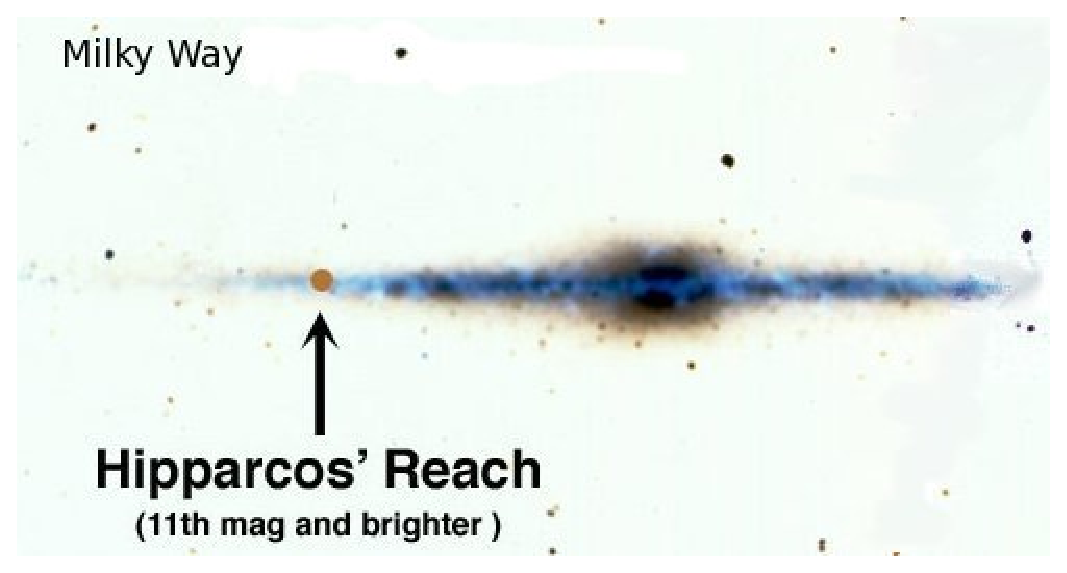
\includegraphics{hippinv}
%\caption{ }\label{fig:erptsqfit}
\end{figure}



Activate the \texttt{Hipparcos-Stars} plugin in Google Sky, this will mark stars that were observed by the Hipparcos satellite. 
Click on 20 stars with a range of colors and record the given absolute magnitude and the B-V color (BV index) for each star to an excel spreadsheet.
 Make the CMD of these stars.
Note that color is a equivalent to a temperature scale that is roughly logarithmic. Similarly magnitudes are logarithmic, so you are looking at stars over a huge range of temperature and brightness. 

 Label the directions of redder color, and higher temperatures on the x-axis. Label higher luminosity on the Y-axis.
 Label the Main Sequence and draw an arrow in the direction stars would go as they evolve off the main sequence into red giants. Label where the massive stars, typical stars and low mass stars sit on the main sequence. Circle the stars that evolve off the main sequence fastest.

 Now zoom out so that you can see hundreds of Hipparcos stars, and turn on the \texttt{Hipparcos-HR} plugin. You should see something similar to the diagram you just created in the left corner. 
Move around the sky and the diagram incorporates the new stars that are now part of your field of view.
 Does the HR diagram change much as you move? Why?
 If more distant disk stars were incorporated in the diagram, would it change? 
Where is the main sequence turn off? What does that tell you about the age of the stellar population you're looking at?
 Approximately how wide is the main sequence? 
 If all stars were exactly the same age, how would the shape of the CMD change? the width?
 If star formation in the disk ceased a long time ago, how would the main sequence change? 





\section*{Determining some of the Properties of a Cluster}

You are now going to try to characterize clusters of stars using data from the SDSS. Deactivate the \texttt{Hipparcos-HR} and \texttt{Hipparcos-Stars} plugins, pan to the SDSS footprint, and zoom in so that you only see a few hundred stars. Activate the \texttt{SDSS-star-hr} plugin to plot an HR-diagram of the 1000 brightest SDSS stars in your field of view. Activate the \texttt{SDSS-star} plugin to see which stars are being included in the diagram. Unlike the Hipparcos catalog SDSS does not have distances to stars, so the \textbf{y-access is apparent magnitude}. Why is there no main sequence in your random field of stars? 


Now we will try to determine the properties of some star clusters. Load their locations by opening \texttt{globular-clusters-coords} and \texttt{open-clusters-coords}. First, check out the open clusters NGC 2420 and M67. You may need to zoom in so that dimmer stars are included in the HR diagram. 
\begin{enumerate}
\item Estimate the distance to the cluster using the HR-diagram. The solar color and R-band apparent magnitude are 
$(G-R)_{sun}$=.9
$m_{Rsun}$=4.5  
and the equation relating distance to magnitude is 
$\frac{D_{cgal}}{D_{sun}}=10^{0.4(m_{cgal}-m_{Rsun})}$

\item How thick is the main sequence, and how does this compare to the Hipparcos disk stars? Why is this?
\item Are these stars from a single age population? Why?
\item Note the general appearance of the clusters, how compact do they appear? Are the stars symmetrically distributed?
\end{enumerate}


\noindent Now read the following questions and then take a look at the globular clusters. 
\begin{enumerate}
\item Note the general appearance of the clusters, how compact do they appear compared to the open clusters? Are the stars symmetrically distributed relative to the open clusters? How does this fit with your understanding of what open/globular clusters are?
\item For M5 and M3 estimate a distance by extrapolating the main sequence if necessary. (If you are out of time note that a 2.5 magnitude increase corresponds to an increase in distance by a factor of 10 and make a quick guess based on your open cluster distances.)
\item How does the age of a population relate to the color of the main sequence turnoff? Order pal5, M3 and M5 by the age of their oldest stars using the Main Sequence turnoff. Can you think of how dust might affect your results? 
%,NGC 5466, M 53, NGC 5053
%pal5=11.5Gyr, N2420=2Gyr, 5466=12.5+-.9, M53=13, 5053=12.5, M3=11, M5=13.5
\item A much more reliable indicator of cluster ages turns out to be the magnitude difference between the main sequence turnoff and the position of the horizontal branch, because both are dimmed by dust in the same way. A larger difference indicates an older population. Rank M3 and M5 using this method did you get the right answer the first time?     
\end{enumerate}

\noindent Finally let's look at some dwarf galaxies in the Milky Way.  Load their locations by opening \texttt{dsph-coords}. Note the appearance of the first three. Do you see any structure in the CMD? Can you see the last two by eye? What about in the HR diagram? What features do you see?

%\begin{center}
%\begin{tabular}{lll}\hline\hline
%%retrieved from http://www.galaxyzooforum.org/index.php?topic=272726.0 
%Name&R.A.&Dec.\\
%&degrees&degrees\\
%NGC 2419&&\\
%NGC 4147&&\\
%NGC 5466&&\\
%NGC 5053&&\\
%M 3&&\\
%M 5&&\\
%NGC 5024/M53&&\\
%M 13 (Hercules)&&\\
%pal 5 & 229.025276& -0.16356829\\
%%pal 3/Sextans C & 151.38148673 & 0.07131903\\
%%M92&&\\
%%M15&&\\
%%NGC 6229&&\\
%%M2&&\\
%%(other names for commented NGC 6341&&\\ %NGC 7078&&\\ %NGC 7089&&\\ %NGC 6205&&\\ %NGC 5904&&\\ %NGC 5272&&\\)
%&&\\
%NGC 2682 / Messier 67&&\\ %M67& 132.8615&11.8114\\
%NGC2420&&\\
%%Beehive Cluster / M44 / Praesepe&&\\
%%DoDz5 587733608017101724&&\\
%%DoDz6 58772975274465763617&&\\
%%Upgren1 587738950414958642&&\\
%%Melotte 111 587741725506077538&&\\
%%(other names for commented pal 4&&\\ %pal 14&&\\)
%
%\end{tabular}
%\end{center}



\end{document}


%You may find the following table of star colors versus temperature
%spectral type useful:
%
%\begin{center}
%\begin{tabular}{llllllllllll}\hline
%Spectral Type&O5&B0&B5&A0&A5&F0&F5&G0&G5&K0&K5\\
%g-r color&-0.11&-0.07&0.06&0.21&0.34&0.48&0.63&0.78&0.90&1.09&1.37\\
%\end{tabular}
%\end{center}
